\documentclass{article}
\usepackage[utf8]{inputenc}
% separazione delle colonne
\usepackage[nosf]{kpfonts}\usepackage{multicol}
\usepackage[document]{ragged2e}
\usepackage{graphicx}
\setlength{\columnsep}{1cm}
\usepackage{tabularx}

\allowdisplaybreaks %% Fix per gli spazi bianchi giganteschi

% margini della pagina
\usepackage{amsmath}
\usepackage[a4paper, total={20cm, 25cm}]{geometry}

\title{Formulario Fisica}
\author{Adrian Castro \and Alessandro Ferrenti}
\date{July 2018}

\begin{document}

\maketitle

\begin{multicols}{3}

%%
\section{Trigonometria}
\begin{gather*}
 \tan (\alpha) = \frac{\sin \alpha}{\cos \alpha} \\
 \cot (\alpha) = \frac{\cos \alpha}{\sin \alpha} \\
 \sin (\alpha) \cos (\alpha) = \sin (2 \alpha)
\end{gather*}

%%
\section{Unità di misura}

\begin{gather*}
1 \cdot N = 1kg \cdot 1 \frac{m}{s^2} \\
1 \cdot \frac{m}{s} = 3.6 \cdot \frac{km}{h} \\
1 \cdot \frac{km}{h} = \frac{1}{3.6} \cdot \frac{m}{s}
\end{gather*}

%%
\section{Vettori}

\begin{gather*}
    \vec{v} = \begin{cases}
     v_x = v \cdot \cos \alpha \\
     v_y = v \cdot \sin \alpha
    \end{cases} \\
    \vec{v} = \vec{v}_x + \vec{v}_y \\
    v = \sqrt{v_x^2 + v_y^2} \\
    \tan \theta = \frac{v_y}{v_x} \\
    \theta = \arctan (\frac{v_y}{v_x})
\end{gather*}

%%
\section{Costanti}

\begin{gather*}
\text{Forza di gravità: } g_{Terra} = 9.81 \frac{m}{s^2} \\
\text{Forza di gravità lunare: } g_{Luna} = 1.62 \frac{m}{s^2} \\
\end{gather*}

%%
\section{Cinematica}
%%
\subsection{Moto rettilineo}
\begin{gather*}
\text{Variazione di velocità: } \Delta v = v - v_0 \\
\text{Tempo trascorso: } \Delta t = t - t_0 \\
\text{Distanza percorsa: } \Delta s = \left| s - s_0 \right| \\
\end{gather*}
\subsection{Moto circolare uniforme}
\textbf{Nota bene: } questo sistema si usa spesso e volentieri per il moto uniforme
\begin{gather*}
\begin{cases}
    v = v_0 + a_t \\
    s = s_0 + v_0 t + \frac{1}{2} a t^2
\end{cases}
\\
\text{Accelerazione:} \\
\begin{cases}
 a = g = 9.81 m/s^2 & \text{Caduta libera} \\
 a = -g = - 9.81m/s^2 & \text{Lancio verso l'alto}
\end{cases}
\\
\text{Velocità: } v = v_0 + a t \\
\text{Tempo: } t = \frac{v - v_0}{a} \\
\text{Accelerazione: } a = \frac{v - v_0}{t} \\
\text{Accelerazione: } a = \frac{2 (s - s_0 - v_0 t)}{t^2} \\
\text{Velocità(senza t): } v = \sqrt{v_0^2 + 2 a (s - s_0)} \\
\text{Posizione: } s = s_0 + v_0 t + \frac{1}{2} a t^2 \\
\text{Posizione(senza a): } s = s_0 + \frac{v + v_0}{2} t \\
\text{Velocità(senza a): } v = \frac{2 (s - s_0)}{t} - v_0
\end{gather*}
%%%
\subsection{Moto parabolico}
\textbf{Nota bene: } l'accelerazione($g$)è negativa quando si presume di partire dal basso verso l'alto, perché la gravita agisce contro il movimento verticale. \\ Al contrario, se ci troviamo in un movimento che parte dall'alto verso il basso, l'accelerazione($g$)sarà positiva!
\begin{gather*}
\text{Equazione parabola: } \begin{cases}
    x = x_0 + v_{0x} t \\
    y = y_0 + v_{0y} t - \frac{1}{2} g t^2
\end{cases}
\\
\text{Equazione parabola: } y = \frac{v_x}{v_y} x - \frac{1}{2} \frac{g}{v_x^2} x^2 \\
\text{Velocità iniziale: } v_0 = \sqrt{v_x^2 + v_y^2} \\
\text{Velocità iniziale: } \begin{cases}
    v_{0x} = v_0 \cos \alpha  = v_y \frac{\cos \alpha}{\sin \alpha} \\
    v_{0y} = v_0 \sin \alpha = v_x \frac{\sin \alpha }{\cos \alpha}
\end{cases}
\\
\text{Velocità(tempo t): } \begin{cases}
    v_x = v_0 \cos \alpha \\
    v_y = v_0 \sin \alpha - a t
\end{cases}
\\
\text{Vertice: } \begin{cases}
    x_v = \frac{v_x v_y}{g} = \frac{v_0^2 \sin (2\alpha)}{g} \\
    y_v = \frac{v_y^2}{2g}
\end{cases}
\\
\text{Gittata: } \frac{v_x v_y}{\frac{1}{2}g} = \frac{v_0^2 \sin (2 \alpha)}{\frac{1}{2}g} \\
\text{Tempo di volo: } t = \frac{v_0 \sin \alpha}{2g} \\
\text{Altezza massima: } y = \frac{v_0^2 \sin (2 \alpha)}{2g}
\end{gather*}

%%%
\subsection{Moto circolare}
\begin{center}
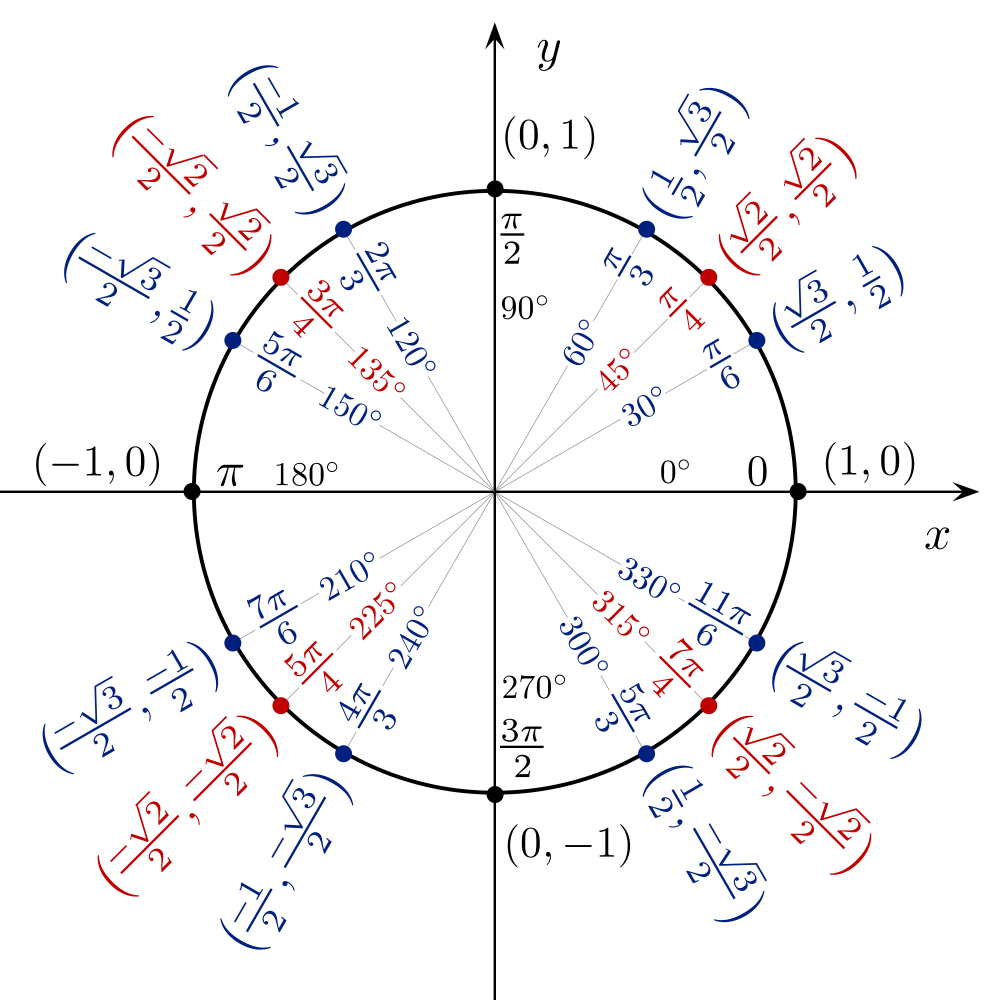
\includegraphics[width=0.8\linewidth]{Cinematica/circonferenza-goniometrica.png}
\end{center}
%%%%
\begin{center}
\begin{tabular}{ c c c }
    Grandezze & Lineari & Angolari \\
    Posizione & $s$ & $\theta$ \\
    Velocità & $v$ & $\omega$ \\
    Accelerazione & $a$ & $\alpha$ \\
\end{tabular}
\end{center}
\textbf{Nota bene: } come la tabella sopra ci indica, c'è una corrispondenza tra grandezze lineari e grandezza angolari. \\ Ciò significa che possiamo immaginare il punto che si muove sulla circonferenza come se si muovesse su una retta(la circonferenza \textit{spiaccicata}), e di conseguenza utilizzare le formule del moto rettilineo per trovarne la posizione!
\begin{gather*}
    \text{Velocità: } v = v_0 + a t \\
    \text{Tempo: } t = \frac{v - v_0}{a} \\
    \text{Accelerazione: } a = \frac{v - v_0}{t} \\
    \text{Posizione: } s = s_0 + v_0 t + \frac{1}{2} a t \\
\end{gather*}
\subsubsection{Moto circolare uniforme}
\textbf{Nota bene: } La velocità tangenziale($v$) indica quanto velocemente il punto si sposta sulla circonferenza($r$); \\
La velocità angolare($\Omega$) indica quanto velocemente cambia l'angolo($\theta$) che il punto forma
\begin{gather*}
\text{Velocità: } v = \frac{\Delta s}{\Delta t} = \frac{2 \pi r}{T} = \omega r = \sqrt{a_c r} \\
\text{Raggio: } r = \frac{v T}{2 \pi} = \frac{v}{\omega} = \frac{v^2}{a_c} = \frac{a_c}{\omega^2} \\
\text{Periodo: } T = \frac{2 \pi r}{v} = \frac{2 \pi}{\omega} \\
\text{Velocità angolare: } \omega = \frac{v}{r} = \frac{2 \pi}{T} = \sqrt{\frac{a_c}{r}} \\
\text{Accelerazione centripeta: } a_c = \frac{v^2}{r} = \omega^2 r \\
\text{Posizione angolare: } \theta = \frac{s - s_0}{r} \\
\textbf{Legge oraria} \\
\text{Posizione angolare: } \theta(t) = \theta_0 + \omega t \\
\text{Velocità angolare: } \omega = \frac{\theta - \theta_i}{t - t_i}
\end{gather*}
%%%%
\subsubsection{Moto circolare uniformemente accelerato(MCUA)}
\textbf{Nota bene: } L'accelerazione centripeta($\vec{a}_c$) permette al punto di mantenere la propria traiettoria sulla circonferenza. Cambia il verso, ma non il modulo della velocità($\vec{v}$) \\
L'accelerazione tangenziale($\vec{a}_T$, perpendicolare a $\vec{a}_c$) invece fa variare il modulo della velocità($\vec{v}$), è \textbf{costante}. \\
L'accelerazione totale($\vec{a}_{tot}$) è la risultante delle accelerazioni precedenti \\
\begin{gather*}
\text{Accelerazione totale: } \vec{a}_{tot} = \vec{a}_T + \vec{a}_c \\
\text{Accelerazione totale: } a_{tot} = \sqrt{a_T^2 + a_c^2} \\
\text{Accelerazione angolare: } \alpha = \frac{d \omega}{d t} = \frac{\omega - \omega_0}{t - t_0} \\
\text{Accelerazione tangenziale: } a_T = \alpha \cdot r \\
\textbf{Legge oraria} \\
\begin{cases}
    \theta = \theta_0 + \omega_0 t + \frac{1}{2} \alpha t^2 & \text{Posizione angolare} \\
    \omega = \omega_0 + \alpha t & \text{Velocità angolare}
\end{cases} \\
\text{Velocità angolare(senza t): } \\ \omega^2 = \omega_0^2 + 2 \alpha(\theta - \theta_0)
\end{gather*}
\subsubsection{Esempio}
\textbf{Nota bene: } per risolvere un problema del tipo: punto materiale con MCUA con $r = 1m$, $s_1 = 0.4m$, $t_1 = 2s$, $t_2 = 4s$, e $v_0 = 0.1 \frac{m}{s}$ dove chiede modulo dell'accelerazione totale al tempo $t_2$(quindi $a_{tot(2)} = \sqrt{a_T^2 + a_{c(2)}^2}$) possiamo impostare il seguente sistema:
\begin{gather*}
    \begin{cases}
        a_{tot(2)} = \sqrt{a_T^2 + a_{c(2)}^2} \\
        a_T = \frac{2(s - s_0 - v_0 t)}{t^2} \\
        a_{c(2)} = \frac{v_2^2}{r} \\ 
        v_{2} = v_0 + a_T \cdot t_2
    \end{cases}
\end{gather*}

%%
\section{Dinamica}

\subsection{Principi fondamentali}

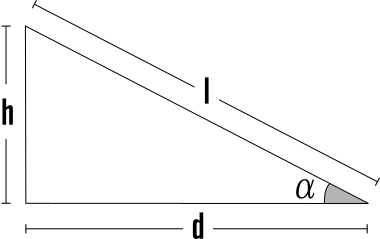
\includegraphics[width=0.4\linewidth]{Dinamica/piano-inclinato-senza-angolo.png} \\

\begin{gather*}
\text{Secondo principio: }
\begin{cases}
    \vec{F} = m \vec{a} \\
    \vec{a} = \frac{\vec{F}}{m} \\
    m = \frac{\vec{F}}{a}
\end{cases} \\
\text{Terzo principio: } \vec{F}_{AB} = -\vec{F}_{BA} \\
\text{$\alpha$(altezza, lunghezza): }\sin{\alpha} = \frac{h}{l} \\ 
\text{$\alpha$(base, lunghezza): }\cos{\alpha} = \frac{d}{l} \\
\text{$\alpha$(altezza, base): }\tan{\alpha} = \frac{h}{d} \\
\end{gather*}
\subsection{Piano inclinato}
\begin{gather*}
    F_{P, x} = F_P \sin (\alpha) = m g \sin (\alpha) \\
    F_{P, y} = F_P \cos (\alpha) = m g \cos (\alpha) 
\end{gather*}
%%%
\subsubsection{Piano inclinato senza attrito}
Piano inclinato: \\
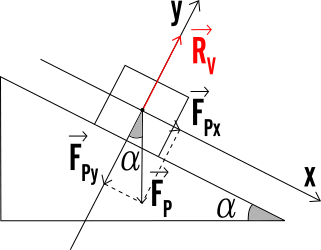
\includegraphics[width=0.75 \linewidth]{Dinamica/reazione-vincolare-nel-piano-inclinato.png} \\
\begin{gather*}
\text{Accelerazione}: \begin{cases}
    a_y = 0 \\
    a_x = g \sin{\alpha}
\end{cases}
\end{gather*}

\subsubsection{Piano inclinato con F verso l'alto}
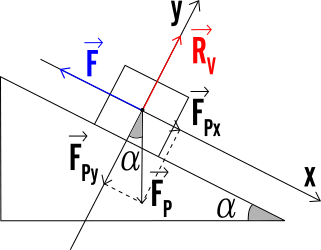
\includegraphics[width=0.75 \linewidth]{Dinamica/variante-piano-inclinato-senza-attrito.png} \\
\textbf{Nota bene: } sull'asse y la forza($F$)che spinge l'oggetto verso l'alto non fa cambiare niente. Ricordiamo che abbiamo scelto \textbf{il piano inclinato} come asse del nostro sistema di riferimento.
\begin{gather*}
    \text{Forza risultante: } F_{ris} = F_{P, x} - F \\
    \text{Accelerazione: } a = \frac{F_{ris}}{m} \\
    \begin{cases}
        F_{P, x} > F & \text{Corpo scende, $a$ positiva} \\
        F_{P, x} < F & \text{Corpo sale, $a$ negativa}
    \end{cases}
\end{gather*}
%%%
\subsubsection{Piano inclinato con attrito}
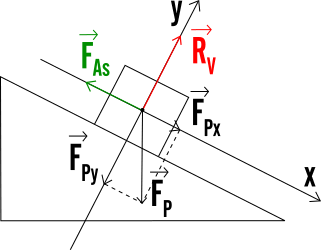
\includegraphics[width=0.75 \linewidth]{Dinamica/piano-inclinato-con-attrito.png} \\
\begin{gather*}
    \text{Forza risultante: } F_{ris, x} = \sqrt{F_{P, x}^2 + F_{As}^2}
\end{gather*}
\textbf{Nota bene: } la forza d'attrito ($F_{A}$, attrito statico nell'immagine) ha verso opposto alla componente della forza peso sull'asse x($F_{P, x}$)
\subsubsection{Attrito Statico}
\begin{gather*}
    \text{Forza Attrito Statico: } \\ F_{As} = \mu_s \cdot F_\perp = \mu_s \cdot F_{P, y} = \mu_s m g \cos (\alpha) \\
    \text{Accelerazione: } \\ a = a_x = g \sin (\alpha) - \mu_s g \cos (\alpha) \\
    \text{Angolo critico per l'equilibrio: } \\ \alpha = \arctan (\mu_s)
\end{gather*}
\subsubsection{Attrito Dinamico}
\textbf{Nota bene: } Per poter considerare il problema dal punto di vista dell'attrito dinamico($\mu_d$)
\begin{gather*}
    \text{Accelerazione: } \\ a = a_x = g \sin (\alpha) - \mu_d g \cos (\alpha)
\end{gather*}

%%
\section{Fluidodinamica}

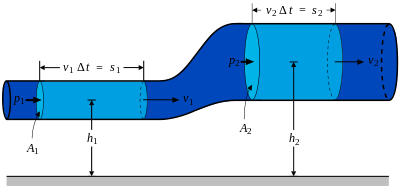
\includegraphics[width=1 \linewidth]{FluidoDinamica/flusso.png} \\

\begin{gather*}
    \textbf{Densità(massa volumica): } \rho = \frac{m}{V} \\
    \textbf{Massa: } m = \rho V \\
    \textbf{Volume: } V = \frac{m}{\rho} \\
    \textbf{Pressione: } p = \frac{F_\perp}{S} \\
    \textbf{Pressione Fluidi Comprimibili: } \\ p = p_0e^{-\frac{\rho_0 g}{p_0}z} \\
    \textbf{Pressione atm. ad altitudine $z$: } \\
    p = p_0e^{-\frac{z}{8006km}} \\
    \textbf{Legge di Stevino: } p = \rho g h \\
    \textbf{Principio di Pascal: } \\ p_1 = p_2 \\ \frac{F_1}{S_1} = \frac{F_2}{S_2} \\
    \textbf{Principio di Archimede: } \\ F_A = P_{fl} = m_{fl} g = \rho_{fl} V_{imm} g \\ \begin{cases}
        \rho_{corpo} > \rho_{fluido} & \text{corpo affonda} \\
        \rho_{corpo} < \rho_{fluido} & \text{corpo in equilibrio} \\
        \rho_{corpp} > \rho_{fluido} & \text{corpo galleggia}
    \end{cases} \\
    \textbf{Formula del galleggiamento: } \\ F_A = F_P \\ \rho_{liq} V_{imm} = \rho_{corpo} V_{tot} \\
    \textbf{Portata: } \\ Q = \frac{V}{\Delta t} \\ Q = A \cdot v \\
    \textbf{Teorema di Bernoulli: } \\ p_1 + \frac{1}{2} \rho v_1^2 + \rho g h_1 = p_2 + \frac{1}{2} \rho v_2^2 + \rho g h_2 \\
    \textbf{Equazione di Continuità(ideale): } \\  Q = v_1 S_1 = v_2 S_2 \\
    \textbf{Equazione di Continuità(reale): } \\ Q = \rho_1 v_1 S_1 = \rho_1 v_2 S_2 \\
    \textbf{Velocità 1: } v_1 = \frac{Q}{S_1} = \frac{S_2}{S_1} v_2 \\
    \textbf{Velocità 2: } v_2 = \frac{Q}{S_2} = \frac{S_1}{S_2} v_1 \\
    \textbf{Sezione 1: } S_1 = \frac{v_2}{v_1} S_2 \\
    \textbf{Sezione 2: } S_2 = \frac{v_1}{v_2} S_1 \\\
    \textbf{Differenza di pressione: } \\
    \Delta p = \frac{1}{2} \rho (v_2^2 - v_1^2) \\ 
    \Delta p = \frac{1}{2} \rho (\frac{Q^2}{S_2^2} - \frac{Q^2}{S_1^2})
\end{gather*}

\end{multicols}

\end{document}